\documentclass[12pt]{article}
\usepackage[utf8]{inputenc}
\usepackage{amsmath, amsfonts, amssymb}
\usepackage{geometry}
\usepackage{graphicx}
\usepackage{hyperref}
\usepackage{algorithm}
\usepackage{algpseudocode}
\usepackage{setspace}

\geometry{margin=1in}

\makeatletter
\def\expinput#1{\@@input#1 }
\makeatother

\begin{document}

\begin{titlepage}
    \centering
    \vspace*{1in}
    \huge
    \textbf{Implementation and Comparative Analysis of Pathfinding Algorithms}\\[0.5in]
    \Large
    \textbf{Author:}\\[0.2in]
    Tanner Wagner\\
    Jennifer Diaz\\
    Odysseus Valdez\\
    Jubilation Megill\\[1in]
    \normalsize
    8 December 2024
    \vfill
\end{titlepage}

\newpage
\tableofcontents
\newpage

\section{Introduction}
Pathfinding algorithms are a cornerstone of computer science and artificial intelligence, finding applications in a wide range of domains such as robotics, video games, and navigation systems. This project aims to explore the implementation and comparative analysis of five fundamental pathfinding algorithms: \textbf{A*}, \textbf{Breadth-First Search (BFS)}, \textbf{Depth-First Search (DFS)}, \textbf{Dijkstra's Algorithm}, and \textbf{Floyd-Warshall Algorithm}. Each of these algorithms is studied in the context of a grid-based environment with varying levels of complexity, obstacles, and goals.
\\
\\
The objective of this report is to:
\begin{itemize}
    \item Provide a clear and concise explanation of each algorithm, including its formal definition, theoretical time and space complexity, and practical implementation.
    \item Demonstrate the performance of these algorithms across multiple test cases, each designed to highlight specific characteristics and challenges inherent to grid-based pathfinding.
    \item Present a comparative analysis of the algorithms, focusing on their execution time, memory usage, and behavior relative to their theoretical complexities.
    \item Discuss coding complexity, debugging efforts, and the observed strengths and weaknesses of each algorithm in different scenarios.
\end{itemize}

\noindent The report is organized as follows:
\begin{itemize}
    \item \textbf{Algorithm Descriptions and Implementations:} Detailed descriptions and pseudocode for each of the five algorithms, including explanations of key concepts such as heuristics, priority queues, and adjacency matrices.
    \item \textbf{Performance Analysis:} A discussion of the algorithms' execution times, memory usage, and overall behavior based on the generated outputs and test cases.
    \item \textbf{Comparative Analysis and Insights:} Insights into why certain algorithms outperform others in specific scenarios and how theoretical complexities translate into actual performance.
    \item \textbf{Conclusion:} A summary of the findings, highlighting the key takeaways from the project and the practical implications of the results.
    \item \textbf{Extra Credit:} An isolated section focusing entirely on the extra credit question and the changes it makes to the algorithm and its output.
    \item \textbf{Team Member Acknowledgements:} A list of all team members and their individual contributions to the project as a whole.
    \item \textbf{Bibliography:} A list of all sources consulted during the project, including foundational texts and course materials.
\end{itemize}

\noindent Through this project, we aim to deepen our understanding of the underlying mechanics of these algorithms and their practical trade-offs, providing a comprehensive evaluation of their suitability for different types of pathfinding problems. Whether the task involves finding a single shortest path, navigating through multiple goals, or solving all-pairs shortest path problems, this report offers an in-depth exploration of the methods and their applications.
\newpage














\section{Tanner Wagner: $A^*$ Algorithm}

\subsection{Introduction to $A^*$}
The A\* algorithm is a widely used pathfinding and graph traversal algorithm that efficiently finds the shortest path between nodes in a weighted graph. It combines the strengths of Dijkstra's algorithm and Greedy Best-First Search by utilizing heuristic functions to guide its search, making it both optimal and efficient in many applications.

\subsection{Formal Definition}
Let \( G = (V, E) \) be a finite graph, where:

\begin{itemize}
    \item \( V \) is the set of vertices (nodes).
    \item \( E \) is the set of edges connecting the vertices.
\end{itemize}

\noindent Each edge \( (u, v) \in E \) has an associated non-negative cost \( c(u, v) \), representing the cost to move from node \( u \) to node \( v \).

\subsection{Objective}
Given:
\begin{itemize}
    \item A start node \( s \in V \).
    \item A goal node \( g \in V \).
    \item A heuristic function \( h: V \rightarrow \mathbb{R}_{\geq 0} \) that estimates the cost from a node to the goal.
\end{itemize}

\noindent Find the path \( P^* \) from \( s \) to \( g \) that minimizes the total cost:
\[
P^* = \arg\min_{P} \left( \sum_{i=0}^{n-1} c(v_i, v_{i+1}) \right)
\]
\noindent where \( P = (v_0, v_1, \dots, v_n) \) is a path such that \( v_0 = s \) and \( v_n = g \).

\subsection{Algorithm Description}
The A\* algorithm maintains the following for each node \( v \):
\begin{itemize}
    \item \( g(v) \): the cost from the start node \( s \) to node \( v \).
    \item \( h(v) \): the heuristic estimate from node \( v \) to the goal node \( g \).
    \item \( f(v) = g(v) + h(v) \): the estimated total cost of a solution path passing through \( v \).
\end{itemize}

\subsection{Algorithm Steps}
\begin{enumerate}
\item \textbf{Initialize}
  \begin{itemize}
    \item Set \( g(s) = 0 \).
    \item Add \( s \) to the open set \( O \) (priority queue) ordered by \( f \)-value.
    \item The closed set \( C \) is initialized as empty.
  \end{itemize}
\item \textbf{Loop}
  \begin{enumerate}
    \item While \( O \) is not empty:
        \begin{enumerate}
            \item Remove the node \( v \) from \( O \) with the lowest \( f(v) \).
            \item If \( v = g \), reconstruct and return the path from \( s \) to \( g \).
            \item Add \( v \) to \( C \).
            \item For each neighbor \( u \) of \( v \):
              \begin{itemize}
                \item If \( u \in C \), continue.
                \item Compute tentative score \( g_{\text{tentative}} = g(v) + c(v, u) \).
                \item If \( u \notin O \) or \( g_{\text{tentative}} < g(u) \):
                  \begin{itemize}
                    \item Set \( g(u) = g_{\text{tentative}} \).
                    \item Set \( f(u) = g(u) + h(u) \).
                    \item Set the parent of \( u \) to \( v \).
                    \item If \( u \notin O \), add \( u \) to \( O \).
                \end{itemize}
            \end{itemize}
        \end{enumerate}
  \end{enumerate}
  \item \textbf{Failure}
    \begin{itemize}
        \item If \( O \) is empty and the goal has not been reached, return failure.
    \end{itemize}
\end{enumerate}

\subsection{Heuristic Function}
The heuristic function \( h(v) \) must satisfy:
\begin{itemize}
    \item \textbf{Admissibility}: It never overestimates the actual minimal cost from \( v \) to \( g \).
    \item \textbf{Consistency (Monotonicity)}: For every edge \( (v, u) \), the estimated cost satisfies
      \[
      h(v) \leq c(v, u) + h(u).
      \]
\end{itemize}

\noindent For grid-based pathfinding without diagonal movement, the \textbf{Manhattan distance} is used:
\[
h(v) = |x_v - x_g| + |y_v - y_g|
\]
\noindent where \( (x_v, y_v) \) and \( (x_g, y_g) \) are the coordinates of node \( v \) and the goal node \( g \), respectively.

\subsection{Algorithm Implementation Details}
In my implementation for a grid-based environment:

\begin{itemize}
    \item \textbf{Grid Representation}:
    \begin{itemize}
        \item The environment is a 2D grid where each cell is either empty or contains an obstacle.
        \item Movements are allowed in four directions: up, down, left, and right.
    \end{itemize}
    \item \textbf{Data Structures}:
    \begin{itemize}
        \item \textbf{Open Set} \( O \): A priority queue implemented as a min-heap, ordered by \( f(v) \).
        \item \textbf{Closed Set} \( C \): A set containing nodes that have already been evaluated.
        \item \textbf{Parents Map}: A mapping from each node to its parent node, used for path reconstruction.
    \end{itemize}
    \item \textbf{Handling Multiple Items}:
    \begin{enumerate}
        \item Find the shortest path to the nearest item using A\*.
        \item Update the start position to the item's location.
        \item Remove the collected item from the list of items.
        \item Repeat until all items are collected.
    \end{enumerate}
    \item \textbf{Path Reconstruction}:
    \begin{itemize}
        \item Once the goal is reached, the path is reconstructed by tracing back from the goal node to the start node using the parents map.
    \end{itemize}
\end{itemize}

\subsection{Time and Space Complexity}
The theoretical time complexity of the A\* algorithm in the worst case is \( O(|E| + |V|\log |V|) \), where \( |E| \) is the number of edges and \( |V| \) is the number of vertices. For a grid of size \( N \times N \):
\[
|V| = N^2 \quad \text{and} \quad |E| = O(N^2)
\]
\\
\noindent Thus, the worst-case time complexity becomes:
\[
O(N^2 \log N)
\]
\\
\noindent In practice, the actual performance is often better due to the heuristic guiding the search efficiently towards the goal. The constant factors in the running time are influenced by:
\begin{itemize}
    \item The efficiency of the priority queue implementation.
    \item The quality of the heuristic function.
    \item The branching factor, which is up to 4 in a grid without diagonal movement.
\end{itemize}

\subsection{Coding Complexity and Debugging}
Implementing A\* required careful management of data structures like the open and closed sets and ensuring the heuristic function is admissible and consistent. Debugging efforts focus on verifying that:
\begin{itemize}
    \item The heuristic function is correctly implemented.
    \item The priority queue correctly orders nodes by \( f(v) \).
    \item Path reconstruction accurately retrieves the optimal path.
\end{itemize}

\subsection{Discussion}
The A\* algorithm is a powerful tool for finding the shortest path in grid-based environments. By utilizing an admissible and consistent heuristic, such as the Manhattan distance, the algorithm efficiently navigates through the grid, avoiding obstacles and minimizing the total path cost. The implementation challenges are balanced by the algorithm's optimality and practical efficiency.
\newpage




















\section{Jennifer Diaz: Depth-First Search (DFS) Algorithm}
\subsection{Introduction to DFS}
Depth-First Search (DFS) is a graph traversal algorithm that explores as far as possible along each branch before backtracking. Unlike A*, which uses heuristics to guide its search, DFS is an uninformed search technique that does not guarantee finding the shortest path in weighted graphs. Instead, DFS systematically explores the search space, potentially visiting all reachable vertices.
\\
\\
When applied to a grid-based pathfinding scenario, DFS can find a path between two points if one exists, but it may not be optimal in terms of path cost or length. Nevertheless, DFS is conceptually simple and easy to implement, making it a good baseline for comparison with more sophisticated algorithms.

\subsection{Formal Definition}
Consider the same graph setup \( G = (V, E) \) and cost function \( c(u,v) \) as defined in the A* section. For DFS, we focus on a simple exploration of the graph structure:

\begin{itemize}
    \item We have a start node \( s \in V \) and a goal node \( g \in V \).
    \item The objective is to find \textit{some} path \( P \) from \( s \) to \( g \) if one exists.
\end{itemize}

\noindent Unlike A*, DFS does not maintain a global cost function or heuristic estimate. Its goal is solely to determine reachability and return one valid path if found. The notion of optimality, in terms of path cost or length, is not guaranteed.

\subsection{Algorithm Description}
DFS can be implemented using a stack, either explicitly (with a stack data structure) or implicitly (with recursion). In this implementation, a stack is used explicitly:


\begin{enumerate}
    \item Initialize a stack with the start node \( s \) and an empty path.
    \item Keep a set of visited nodes to avoid revisiting the same state repeatedly.
    \item Pop the top element \((current, path)\) from the stack.
    \item If \( current = g \), return the path found.
    \item Otherwise, expand the neighbors of \( current \) that are not visited and push them onto the stack with the updated path.
    \item Repeat until the stack is empty or the goal is found.
\end{enumerate}

\noindent If the stack empties before reaching \( g \), no path exists.

\subsection{Grid Environment and Multiple Items}
In this project, DFS is applied to a 2D grid environment:
\begin{itemize}
    \item Each cell can be free or contain an obstacle.
    \item Movements are allowed up, down, left, and right.
\end{itemize}

\noindent To handle multiple items, the algorithm:
\begin{enumerate}
    \item Starts at the initial position and attempts to find a path to the first item in the list.
    \item If a path is found, the agent moves along this path, collects the item, updates its current position to the item's location, and then attempts to find a path to the next item.
    \item If at any point no path to the next item exists, the algorithm reports failure.
    \item After all items are collected, the algorithm optionally attempts to return to the start position.
\end{enumerate}

\noindent This sequential approach ensures that DFS tries to solve a series of point-to-point pathfinding problems.

\subsection{Time and Space Complexity}
For a grid of size \( N \times N \):

\begin{itemize}
    \item \textbf{Time Complexity}: In the worst case, DFS may visit every cell. The complexity is \( O(N^2) \) since each cell is visited at most once (due to the visited set). Without weights or heuristics, DFS doesn't prune paths based on cost, so it could explore large portions of the grid.
    \item \textbf{Space Complexity}: DFS stores only the stack and visited set. In the worst case, the visited set may contain all cells, giving a complexity of \( O(N^2) \).
\end{itemize}

\subsection{Coding Complexity and Debugging}
The DFS implementation is straightforward:
\begin{itemize}
    \item No heuristic function is needed.
    \item The primary challenge lies in correctly maintaining a visited set and ensuring the stack operations are implemented correctly.
    \item Debugging is simpler relative to algorithms like A* or Dijkstra's algorithm since there are no priority queues or advanced cost computations.
\end{itemize}

\subsection{Discussion}
DFS provides a baseline for performance comparison. While it can find a path, it may not find the shortest one. In environments where memory is sufficient and optimality is not a priority, DFS can be a simple and fast solution to implement. However, when path cost or distance is critical, DFS is often outperformed by algorithms like A*, which use heuristics to guide the search towards the goal more efficiently.
\newpage









\section{Jennifer Diaz: Breadth-First Search (BFS) Algorithm}
\subsection{Introduction to BFS}
Breadth-First Search (BFS) is a fundamental graph traversal algorithm that explores all neighbors of a node before moving on to the next level of nodes. In an unweighted graph (or grid), BFS is guaranteed to find the shortest path in terms of the number of edges (or moves) from the start to the goal, making it optimal for such scenarios.
\\
\\
When applied to a grid-based environment, BFS can efficiently find the shortest path between two points, assuming uniform step costs. However, like DFS, BFS is uninformed—no heuristic is used. This makes BFS simpler than A*, but less directed. Nonetheless, BFS is often considered a baseline for comparison due to its simplicity and optimality (in unweighted settings).

\subsection{Formal Definition}
As with A* and DFS, consider a grid-based graph \( G = (V, E) \) where:
\begin{itemize}
    \item Each vertex \( v \in V \) corresponds to a cell in the grid.
    \item Each edge \( (u, v) \in E \) represents a valid move from cell \( u \) to cell \( v \).
\end{itemize}

\noindent In BFS, the objective, given a start node \( s \in V \) and a goal node \( g \in V \), is to find the shortest path \( P \) from \( s \) to \( g \) in terms of the number of steps. Since the grid is unweighted and moves have uniform cost, BFS will find a path \( P^* \) that minimizes:
\[
|P^*| = \arg\min_{P \subseteq V} \left( \sum_{i=0}^{n-1} 1 \right)
\]
\noindent Here the cost is essentially the number of moves, each counting as one.

\subsection{Algorithm Description}
BFS typically uses a queue structure to manage frontier nodes:
\begin{enumerate}
    \item Initialize a queue with the start node \( s \), along with a path containing only \( s \).
    \item Maintain a visited set to avoid revisiting nodes.
    \item Dequeue the front element \((current, path)\) from the queue.
    \item If \( current = g \), return the path.
    \item Otherwise, enqueue all unvisited neighbors of \( current \) with their respective paths.
    \item Repeat until the queue is empty or the goal is found.
\end{enumerate}

\noindent If the queue empties before finding the goal, no path exists.

\subsection{Grid Environment and Multiple Items}
In this project, BFS is applied to the same 2D grid environment used by A* and DFS:
\begin{itemize}
    \item Each cell may be free or blocked by an obstacle.
    \item Movements are allowed up, down, left, and right.
\end{itemize}

\noindent For multiple items:
\begin{enumerate}
    \item Start from the initial position, run BFS to find the shortest path to the first item.
    \item Move along that path, collect the item, and set the current position to the item's location.
    \item Proceed to the next item in the list, using BFS again from the new start position.
    \item If any item is unreachable, report failure.
    \item After collecting all items, the algorithm may attempt to return to the start position using BFS once more.
\end{enumerate}

\noindent This sequential approach ensures BFS solves multiple subproblems of point-to-point shortest path queries in an unweighted grid.

\subsection{Time and Space Complexity}
For a grid of size \( N \times N \):
\begin{itemize}
    \item \textbf{Time Complexity}: BFS may in the worst case visit every cell. Each cell is enqueued and dequeued at most once. Hence, the time complexity is \( O(N^2) \).
    \item \textbf{Space Complexity}: BFS stores the queue and visited set. In the worst case, both can grow to include all cells, yielding \( O(N^2) \) space complexity.
\end{itemize}

\noindent Since BFS explores nodes level by level, it is guaranteed to find the shortest path (in terms of moves) in an unweighted scenario.

\subsection{Coding Complexity and Debugging}
BFS is relatively easy to implement:
\begin{itemize}
    \item No heuristic or priority queue is needed.
    \item The primary considerations are maintaining the queue for the frontier nodes and the visited set.
    \item Debugging typically involves ensuring that the queue operations and visited checks function correctly.
\end{itemize}

\subsection{Discussion}
BFS serves as a strong baseline algorithm. While it does not leverage heuristics to reduce search time, it provides guaranteed shortest paths in an unweighted grid. This makes BFS useful as a benchmark for evaluating the performance of more complex algorithms like A*. By comparing BFS results against those of A* or other heuristic-driven methods, we can measure the efficiency and benefits that heuristics provide.
\newpage








\section{Jubilation Megill: Floyd–Warshall Algorithm}
\subsection{Introduction to the Floyd–Warshall Algorithm}
The Floyd–Warshall algorithm is a classic dynamic programming approach that finds shortest paths between all pairs of vertices in a weighted graph. Unlike single-source shortest path algorithms (e.g., BFS, DFS, A*, or Dijkstra’s), Floyd–Warshall simultaneously computes the shortest distance from every node to every other node. This global perspective is especially useful when planning routes that must pass through multiple intermediate points.
\\
\\
In the context of a grid-based environment, Floyd–Warshall:
\begin{itemize}
    \item Converts the grid into a graph where each free cell is a vertex.
    \item Computes the shortest path cost between all pairs of free cells.
    \item Once all-pairs shortest paths are known, it applies a greedy strategy to find an approximate route passing through all required items, starting and potentially returning to the initial position.
\end{itemize}

\noindent This approach is different from other algorithms discussed (like A*, BFS, or DFS), which focus on finding a single path between specified start and goal nodes. Floyd–Warshall, by contrast, provides a complete shortest-path picture of the environment.

\subsection{Formal Definition}
Given a set of vertices \( V \) representing free cells and edges \( E \) representing movements between adjacent cells, the Floyd–Warshall algorithm computes a distance matrix \( D \) such that:
\[
D[i,j] = \text{the shortest path cost from } V_i \text{ to } V_j.
\]
\\
\noindent If the grid has \( N \times N \) free cells, we have:
\[
|V| = N^2 \quad\text{(in the worst case, if no obstacles are present).}
\]
\\
\noindent The Floyd–Warshall algorithm initializes the \( D \) matrix using direct edge costs and then iteratively updates it, considering each vertex as an intermediate node:
\[
D[i,j] = \min(D[i,j], D[i,k] + D[k,j]) \quad \text{for all } i,j,k.
\]
\\
\noindent After completing these updates, \( D[i,j] \) holds the shortest path cost from \( V_i \) to \( V_j \) if one exists, or \(\infty\) otherwise.

\subsection{Algorithm Description}
The Floyd–Warshall steps are:
\begin{enumerate}
    \item Initialize the distance matrix \( D \) so that:
    \begin{itemize}
        \item \( D[i,i] = 0 \) for all \( i \).
        \item \( D[i,j] = 1 \) if an edge (i.e., adjacency) exists between \( V_i \) and \( V_j \).
        \item \( D[i,j] = \infty \) if there is no direct edge between \( V_i \) and \( V_j \).
    \end{itemize}
    \item For each vertex \( k \):
    \[
    \forall i,j: D[i,j] = \min(D[i,j], D[i,k] + D[k,j])
    \]
    This step ensures that every possible intermediate vertex is considered.
\end{enumerate}

\subsection{Planning a Route Through All Items}
Once the all-pairs shortest paths are computed, the algorithm uses a greedy approach to:
\begin{enumerate}
    \item Start from the initial position.
    \item At each step, choose the nearest unvisited item according to the precomputed shortest paths in \( D \).
    \item Move to that item, mark it collected, and repeat until all items are obtained.
\end{enumerate}

\noindent This approach resembles a heuristic solution to a Traveling Salesman Problem (TSP)-like scenario on the grid. While this method does not guarantee the optimal order of item collection, it leverages the global distance information to find a reasonably good route.

\subsection{Time and Space Complexity}
The Floyd–Warshall algorithm runs in:
\[
O(|V|^3)
\]
\\
\noindent For a grid of size \( N \times N \):
\[
|V| = N^2 \implies O((N^2)^3) = O(N^6)
\]
\\
\noindent This is significantly more expensive than single-source algorithms and quickly becomes infeasible for large grids.
\\
\\
\noindent Memory usage is also substantial:
\[
O(|V|^2) = O(N^4)
\]
\noindent space is required to store the distance and predecessor matrices.

\subsection{Coding Complexity and Debugging}
Implementing Floyd–Warshall correctly involves:
\begin{itemize}
    \item Proper initialization of the distance matrix \( D \) and predecessor matrix \( P \).
    \item Carefully handling \(\infty\) values and edge cases.
    \item After computing all pairs shortest paths, implementing a greedy strategy to find a route through all items adds complexity.
\end{itemize}

\noindent Debugging this code can be more challenging due to the multiple nested loops and the complexity of verifying all-pairs shortest paths. Adding or removing a single edge or changing the grid structure can affect many computed distances.

\subsection{Discussion}
Floyd–Warshall stands apart from the other algorithms discussed. Instead of focusing on a single start-goal pair at a time, it calculates the shortest paths for all pairs. This makes it well-suited for situations where multiple queries or multiple intermediate targets exist. However, the high computational cost and memory usage limit its scalability on large grids.
\\
\\
When combined with a heuristic route-planning step (like a greedy approach), Floyd–Warshall can provide a decent solution for collecting items scattered throughout the grid, though it may be overkill or too resource-intensive for simpler pathfinding needs.
\newpage










\section{Odysseus Valdez: Dijkstra's Algorithm}
\subsection{Introduction to Dijkstra's Algorithm}
Dijkstra's algorithm is a classic algorithm for finding the shortest path from a source vertex to all other vertices in a graph with non-negative edge weights. Unlike A*, it does not rely on heuristics but systematically explores nodes in increasing order of distance from the source. In the context of grid-based environments, Dijkstra's algorithm guarantees finding the optimal path to a goal node while handling uniform or varying step costs.


\subsection{Formal Definition}
Let \( G = (V, E) \) be a graph, where:
\begin{itemize}
    \item \( V \) is the set of vertices (nodes), and \( E \) is the set of edges.
    \item Each edge \( (u, v) \in E \) has a non-negative weight \( w(u, v) \), representing the cost to travel from node \( u \) to node \( v \).
\end{itemize}

\noindent Given:
\begin{itemize}
    \item A source node \( s \in V \).
    \item A set of goal nodes \( G = \{g_1, g_2, \dots, g_k\} \subseteq V \).
\end{itemize}

\noindent The objective is to compute the shortest path \( P^* \) from \( s \) to each \( g \in G \) such that:
\[
P^* = \arg\min_P \left( \sum_{(u,v) \in P} w(u,v) \right)
\]
\noindent where \( P \) is a path in \( G \).

\subsection{Algorithm Description}
Dijkstra's algorithm operates by iteratively expanding the shortest known path to unexplored nodes. Key components include:
\begin{itemize}
    \item A priority queue to manage frontier nodes, ordered by their current shortest path estimate.
    \item A distance map \( d[v] \) storing the shortest known distance from \( s \) to \( v \).
    \item A parent map \( p[v] \) to reconstruct paths once the goal is reached.
\end{itemize}

\noindent Steps of the algorithm:
\begin{enumerate}
    \item \textbf{Initialization:}
    \begin{itemize}
        \item Set \( d[s] = 0 \) and \( d[v] = \infty \) for all \( v \in V \setminus \{s\} \).
        \item Add \( (0, s) \) to the priority queue.
    \end{itemize}
    \item \textbf{Main Loop:}
    \begin{itemize}
        \item While the priority queue is not empty:
        \begin{enumerate}
            \item Extract the node \( u \) with the smallest \( d[u] \).
            \item For each neighbor \( v \) of \( u \):
            \begin{itemize}
                \item Compute \( d_{\text{tentative}} = d[u] + w(u, v) \).
                \item If \( d_{\text{tentative}} < d[v] \), update \( d[v] \), set \( p[v] = u \), and add \( v \) to the queue.
            \end{itemize}
        \end{enumerate}
    \end{itemize}
    \item \textbf{Path Reconstruction:}
    \begin{itemize}
        \item Starting from each goal node \( g \in G \), trace back using \( p[v] \) to construct the path from \( s \).
    \end{itemize}
\end{enumerate}

\subsection{Handling Multiple Items}
In this implementation, the algorithm handles multiple items by:
\begin{enumerate}
    \item Running Dijkstra's algorithm from the current position to find the nearest item.
    \item Moving along the shortest path to collect the item.
    \item Updating the current position and repeating until all items are collected.
\end{enumerate}

\subsection{Time and Space Complexity}
For a grid of size \( N \times N \):
\begin{itemize}
    \item \textbf{Time Complexity:} Each node and edge is processed once in the priority queue. Using a min-heap, the complexity is:
    \[
    O(|E| + |V| \log |V|) = O(N^2 \log N) \quad \text{for a grid.}
    \]
    \item \textbf{Space Complexity:} The algorithm stores distances, parents, and the priority queue. Thus, the complexity is:
    \[
    O(N^2)
    \]
\end{itemize}


\subsection{Coding Complexity and Debugging}
Implementing Dijkstra's algorithm required:
\begin{itemize}
    \item Efficiently managing the priority queue with a min-heap.
    \item Properly updating distance and parent maps to avoid redundant calculations.
    \item Correctly handling multiple goals by iteratively updating the source and recomputing paths.
\end{itemize}

\noindent Debugging challenges included:
\begin{itemize}
    \item Verifying correctness of the priority queue operations.
    \item Ensuring no items were left unvisited due to early termination or incorrect updates.
    \item Handling edge cases such as unreachable nodes.
\end{itemize}

\subsection{Discussion}
Dijkstra's algorithm is a powerful and optimal method for shortest-path computation in non-negative weighted graphs. Its deterministic nature and lack of reliance on heuristics make it a reliable baseline for comparison. However, its performance in dense grids, where many nodes are explored, can lag behind heuristic-driven algorithms like A*. The iterative approach for handling multiple items, while effective, may introduce overhead compared to more global solutions such as Floyd–Warshall.
\newpage












\section{Performance Analysis and Discussions}
This section presents a comparative analysis of the implemented pathfinding algorithms based on the generated outputs, performance metrics, and visualized theoretical complexities. 

\subsection{(a) Comparison of Asymptotic Running Times and Actual Performance}
The following bar chart illustrates the average execution time for all algorithms across the test cases:
\begin{figure}[h!]
    \centering
    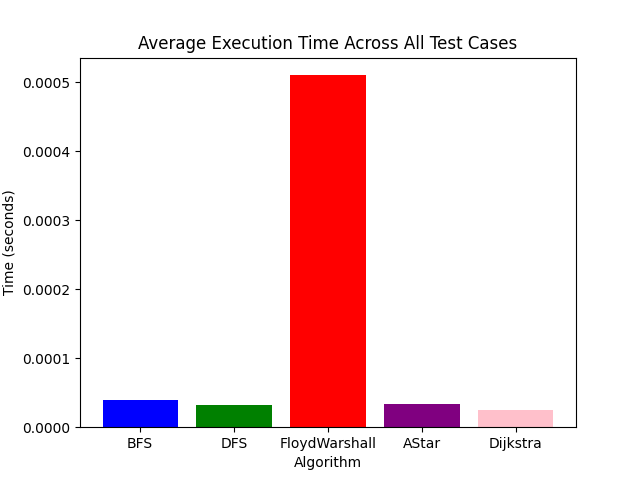
\includegraphics[width=0.8\textwidth]{average_execution_time.png}
    \caption{Average Execution Time Across All Test Cases}
    \label{fig:execution_time}
\end{figure}

\noindent From Figure~\ref{fig:execution_time}, we observe:
\begin{itemize}
    \item Floyd-Warshall is significantly slower than the other algorithms due to its cubic time complexity \( O(|V|^3) \), especially evident with larger grids.
    \item $A^*$, DFS, and Dijkstra exhibit the fastest execution times, followed closely by BFS. The simplicity of BFS and the efficient use of priority queues in Dijkstra allow for optimal performance in these scenarios.
    \item DFS is slightly slower than A*, likely due to its exhaustive exploration of paths without pruning based on a heuristic or cost function.
    \item A* remains efficient but does not outperform Dijkstra in these cases, potentially due to the simplicity of the grid structure and heuristic usage.
\end{itemize}

\noindent The following plot compares the theoretical time complexities:
\begin{figure}[h!]
    \centering
    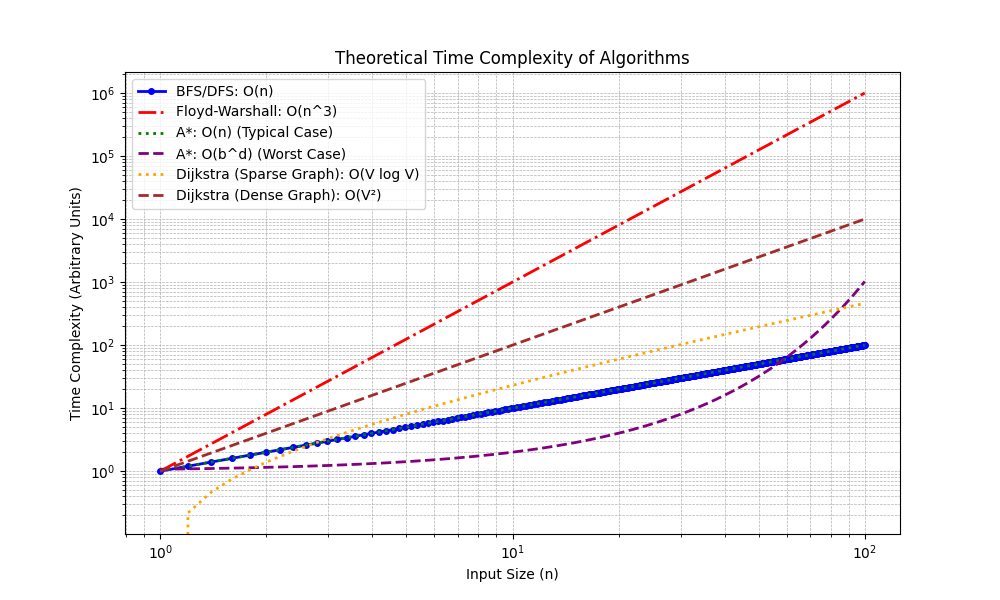
\includegraphics[width=0.8\textwidth]{theoretical_complexities.png}
    \caption{Theoretical Time Complexity of Algorithms}
    \label{fig:theoretical_complexity}
\end{figure}

\noindent The Figure~\ref{fig:theoretical_complexity} aligns well with the observed execution times, emphasizing the dominant cubic growth of Floyd-Warshall and the \( O(|V|^2) \) complexity of Dijkstra on dense graphs.

\subsection{(b) Coding Complexity and Debugging Effort}
The coding complexity and debugging effort vary significantly:
\begin{itemize}
    \item Floyd-Warshall: Debugging was challenging due to the nested loops and managing the distance matrices, but the algorithm itself is straightforward to implement.
    \item BFS and DFS: These were the easiest to code and debug due to their simple structures.
    \item $A^*$ and Dijkstra: Both required intricate data structure management (priority queues). A* added complexity with the heuristic function.
\end{itemize}

\subsection{(c) Fastest and Slowest Algorithms}
Based on the analysis:
\begin{itemize}
    \item \textbf{Fastest:} $A^*$, DFS, and Dijkstra. The combination of simplicity (BFS) and optimal use of priority queues (Dijkstra) allows for excellent performance.
    \item \textbf{Slowest:} Floyd-Warshall. Its cubic complexity and all-pairs shortest path computation make it unsuitable for larger grids.
\end{itemize}

\subsection{(d) Memory Usage and Maximum Grid Size}
The following bar chart illustrates the average number of nodes explored across all test cases, serving as a proxy for memory usage:

\begin{figure}[h!]
    \centering
    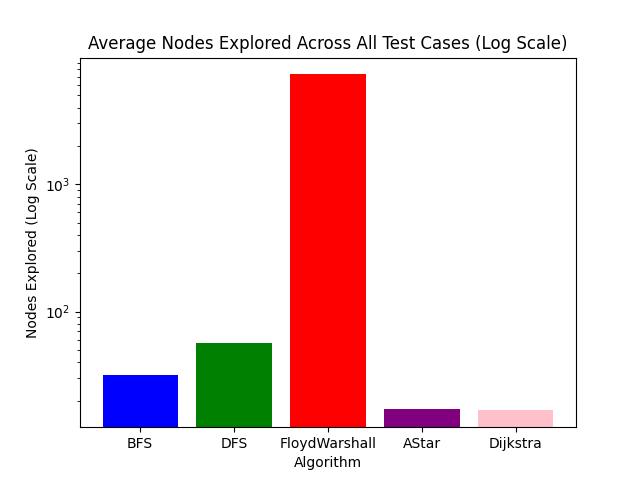
\includegraphics[width=0.8\textwidth]{average_nodes_explored_log.png}
    \caption{Average Nodes Explored Across All Test Cases (Log Scale)}
    \label{fig:nodes_explored}
\end{figure}

\noindent The Figure~\ref{fig:nodes_explored} highlights:
\begin{itemize}
    \item Floyd-Warshall: The most memory-intensive, with thousands of nodes explored due to its global computation.
    \item BFS and DFS: Moderate memory usage due to their straightforward exploration strategies. Though still not as good as $A^*$ and Dijkstra.
    \item A* and Dijkstra: not nearly as much memory usage, attributed to the priority queue and heuristic/map management.
\end{itemize}

\noindent For the current grid size of \( 5 \times 5 \), all algorithms operated without memory issues. However, for larger grids:
\begin{itemize}
    \item BFS, DFS, A*, and Dijkstra are expected to scale better due to their more localized computation.
    \item Floyd-Warshall would likely encounter memory constraints first due to its \( O(N^2) \) memory requirement for the distance matrix.
\end{itemize}

\subsection{Conclusion}
The analysis of the pathfinding algorithms reveals some intriguing discrepancies between their theoretical time complexities and actual performance on the \( 5 \times 5 \) grid test cases. While the theoretical results align with expectations for larger inputs, the small grid size and specific characteristics of the test cases explain some of the observed deviations:

\begin{itemize}
    \item \textbf{Grid Size and Input Characteristics:} The \( 5 \times 5 \) grid is relatively small, minimizing the impact of asymptotic complexities. Algorithms like A* and Dijkstra, which excel on larger inputs due to their efficient handling of complex structures, do not have as much room to showcase their advantages over simpler algorithms like BFS and DFS. In these small grids, the overhead associated with managing priority queues and heuristic functions can outweigh the benefits.
    
    \item \textbf{Heuristic Limitations in A*:} A* heavily relies on the heuristic function to guide its search efficiently. In our test cases, the heuristic (Manhattan distance) might not always provide significant pruning, especially in grids with multiple optimal paths or closely spaced items. As a result, A* sometimes explored a comparable or greater number of nodes than simpler algorithms.

    \item \textbf{BFS and DFS Simplicity:} The relative simplicity of BFS and DFS becomes advantageous in these small grids. These algorithms avoid the overhead of maintaining additional data structures, allowing them to achieve faster execution times in cases where all items or goals are in accessible regions with straightforward paths.

    \item \textbf{Floyd-Warshall's Computational Intensity:} Floyd-Warshall's all-pairs shortest path computation inherently results in higher execution times and memory usage, as expected from its \( O(|V|^3) \) complexity. However, this algorithm's global perspective can be advantageous in scenarios requiring precomputed shortest paths for multiple queries.

    \item \textbf{Dijkstra’s Consistent Efficiency:} Dijkstra's strong performance is a testament to its effective use of priority queues to ensure optimal pathfinding. Its behavior closely mirrors that of A* in these grids, but without the added complexity of heuristic calculations, it occasionally outperformed A*.

    \item \textbf{Simpler Algorithms Surpassing Advanced Ones:} Simpler algorithms like BFS and DFS outperforming advanced ones such as A* in these tests underscore the importance of matching algorithm choice to problem size and complexity. The additional features of advanced algorithms are designed to handle large-scale or highly complex scenarios, which are not present in small grid tests.
\end{itemize}

\noindent In summary, while theoretical complexities provide valuable insights into the behavior of algorithms for large inputs, actual performance can vary significantly based on input size, grid structure, and algorithmic overhead. For small grids, simplicity often prevails, but as grid sizes and complexity grow, the advantages of advanced algorithms like A* and Floyd-Warshall become more apparent.
\newpage


\section{Team Member Acknowledgements}
\subsection{Jennifer Diaz}
Implemented the breadth first search (BFS) and depth first search (DFS) algorithms as well as helped with the full implementation found in Main.py and the report. Additionally, implemented extra credit for BFS and DFS.

\subsection{Jubiliation Megill}
Implemented the algorithm of our choice for this project which ended up being the Floyd-Warshall algorithm. Additionally, helped with the full implementation in Main.py as well as his section of the report. Additionally, implemented extra credit for Floyd-Warshall.

\subsection{Odysseus Valdez}
Implemented Dijkstra's algorithm as well as helped with the full implementation in Main.py and the report. Additionally, implemented extra credit for Dijkstra's algorithm.

\subsection{Tanner Wagner}
Implemented $A^*$ algorithm, helped with full implmentation in Main.py, drafted report, helped with full implementation of comparative analysis in Main.py using numpy as well as implemented extra credit for $A^*$ algorithm.
\newpage




\section{Bibliography}
\begin{enumerate}
    \item Hart, P. E., Nilsson, N. J., \& Raphael, B. (1968). \textit{A Formal Basis for the Heuristic Determination of Minimum Cost Paths}. IEEE Transactions on Systems Science and Cybernetics, 4(2), 100–107.
    \item Russell, S., \& Norvig, P. (2010). \textit{Artificial Intelligence: A Modern Approach} (3rd ed.). Prentice Hall.
    \item Dechter, R., \& Pearl, J. (1985). \textit{Generalized Best-First Search Strategies and the Optimality of A*}. Journal of the ACM, 32(3), 505–536.
    \item Cormen, T. H., Leiserson, C. E., Rivest, R. L., \& Stein, C. (2009). \textit{Introduction to Algorithms} (3rd ed.). MIT Press.
    \item Dijkstra, E. W. (1959). \textit{A Note on Two Problems in Connexion with Graphs}. Numerische Mathematik, 1, 269–271.
    \item Floyd, R. W. (1962). \textit{Algorithm 97: Shortest Path}. Communications of the ACM, 5(6), 345.
    \item Warshall, S. (1962). \textit{A Theorem on Boolean Matrices}. Journal of the ACM, 9(1), 11–12.
    \item Tarjan, R. E. (1972). \textit{Depth-First Search and Linear Graph Algorithms}. SIAM Journal on Computing, 1(2), 146–160.
    \item Course Lecture Notes on Pathfinding Algorithms, CS 361, Fall 2024.
\end{enumerate}
\end{document}
